\chapter{String Theory and M-Theory}

Two promises organize this lecture. We want to understand why gravity appears inside string theory, and we want to see why string theory is far more constrained than the mechanics of point particles. The argument does not begin with grand formalism. It begins with a simpler question: when we describe motion on a curved space by finer and finer approximations, when do the answers settle down to a genuine continuum theory? We follow Leonard Susskind's lecture closely, and these companion notes are prepared from source material credited to Leonard Susskind, LazyingArt LLC, and Video2Book.

\section{From Curved-Space Particles to the String-Theory Question}

Point particles can move perfectly well on smooth curved spaces. Classically the motion is geodesic motion: in the absence of forces tangent to the surface, the particle moves as straight as possible within the surface. One may think of a curved two-dimensional surface, but nothing essential depends on the number of dimensions. The point is simply that ordinary mechanics is comfortable on curved backgrounds.

Susskind then sharpens the issue. A differential equation is already a continuum statement, but in practice one imagines replacing derivatives by finite differences, breaking a trajectory into little pieces, and then taking the limit in which the pieces become arbitrarily fine. For an ordinary point particle on a smooth surface, this limit exists. The classical equations are ordinary differential equations, and in quantum mechanics the corresponding question is controlled by the Schr\"odinger equation or, equivalently, by the path integral. Either way, one finds a sensible continuum theory.

\subsection{Question \& Answer}

\paragraph{Question.} What does it mean for the continuum limit to exist?

\paragraph{Answer.} It means that when we discretize the motion and then refine the discretization, the physical answers stabilize instead of wandering. For a point particle this is exactly what smooth differential equations and their quantum counterparts guarantee. The trajectory, or the transition amplitude, approaches a definite limit as the grain size is taken to zero. This ordinary success story is the control example against which the string will now be measured.

String theory is subtler because the moving object is not a point. It is an extended object, and its extension is not an afterthought: quantum mechanically the string fluctuates, spreads out, and therefore samples the background geometry in a qualitatively different way. To see the difference cleanly, Susskind takes the simplest curved target space he can draw: a sphere.

\section{A Point Particle on a Sphere}

We begin with the point-particle problem on a sphere of radius \(r\). On the board the radius is marked as \(R\); in the formulas below we follow the lecture's spoken notation \(r\).

\begin{figure}[h]
\centering

\includegraphics[width=0.56\textwidth]{lecture_09_figure_02.png}
\caption{Sphere sketch with radius label.}
\end{figure}

\begin{figure}[h]
\centering
\begin{tikzpicture}[scale=1.1]
\draw (0,0) circle (1.9);
\fill (0.15,1.72) circle (1.4pt);
\node at (-0.75,2.22) {$R$};
\end{tikzpicture}
\caption{Minimal redraw of the sphere cross-section used to set up the control problem.}
\end{figure}

The kinetic energy is just the usual one,
\begin{equation}
E=\frac{1}{2}mv^2=\frac{p^2}{2m},
\end{equation}
with the understanding that the momentum vector is tangent to the sphere. Quantum mechanically it is natural to rewrite this in terms of angular momentum. Since the motion is along a great circle, the magnitude of the angular momentum is
\begin{equation}
L=pr.
\end{equation}
Therefore
\begin{equation}
E=\frac{p^2}{2m}=\frac{L^2}{2mr^2}.
\end{equation}
Now \(mr^2\) is the moment of inertia \(I\), so the same expression becomes
\begin{equation}
E=\frac{L^2}{2I}, \qquad I=mr^2.
\end{equation}

This is the entire point-particle control example in a nutshell. The geometry enters through the moment of inertia, the angular momentum is quantized, and ordinary mechanics remains perfectly healthy. Nothing runs away as we refine the description. The sphere is therefore a harmless background for a particle.

\section{Zero-Point Oscillations and the Size of a String}

Now we keep the sphere and replace the point particle by a string constrained to move on that sphere. Susskind immediately asks the right question: how large is the string, even in its ground state? The reason is that a quantum string is never truly rigid or pointlike. Zero-point oscillations give it a fluctuating size.

For simplicity the lecture uses an open string and writes only the structural part of the mode expansion, suppressing factors that are not important for the argument:
\begin{equation}
X(\sigma)-X_{\mathrm{cm}}
\sim
\sum_{n>0}\frac{a_{+n}+a_{-n}}{\sqrt{n}}\cos n\sigma.
\end{equation}
Here \(\sigma\) parametrizes the string, \(X_{\mathrm{cm}}\) is the center-of-mass term, and \(a_{+n}\), \(a_{-n}\) are the creation and annihilation operators in the lecture's notation.

The size is measured by the mean squared separation of a point on the string from the center of mass:
\begin{align}
\left\langle \bigl(X(\sigma)-X_{\mathrm{cm}}\bigr)^2 \right\rangle
&\sim
\sum_{n,m>0}
\frac{
\langle 0|(a_{+n}+a_{-n})(a_{+m}+a_{-m})|0\rangle
}{\sqrt{nm}}
\cos n\sigma \cos m\sigma.
\end{align}
The vacuum expectation value is straightforward once we inspect the operator structure.

\begin{enumerate}
\item Terms of the form \(a_{+}a_{+}\) create excitations and therefore do not overlap with the ground state.
\item Terms of the form \(a_{-}a_{-}\) annihilate the vacuum.
\item The mixed term \(a_{+}a_{-}\) also vanishes in the vacuum expectation value.
\item The only surviving contribution is \(a_{-n}a_{+m}\), and it contributes only when \(n=m\):
\begin{equation}
\langle 0|a_{-n}a_{+m}|0\rangle=\delta_{nm}.
\end{equation}
\end{enumerate}

So the double sum collapses to a single sum,
\begin{equation}
\left\langle \bigl(X(\sigma)-X_{\mathrm{cm}}\bigr)^2 \right\rangle
\sim
\sum_{n>0}\frac{\cos^2 n\sigma}{n}.
\end{equation}
Since \(\cos^2 n\sigma\) is always positive and averages to roughly \(1/2\), the lecture reduces this to the estimate
\begin{equation}
\left\langle \bigl(X(\sigma)-X_{\mathrm{cm}}\bigr)^2 \right\rangle
\approx
\frac{1}{2}\sum_{n>0}\frac{1}{n}.
\end{equation}

This is the first serious warning. The harmonic sum diverges. If we impose a cutoff \(n_{\max}\), then the effective size grows only logarithmically,
\begin{equation}
R_{\mathrm{eff}}^2 \sim \log n_{\max},
\end{equation}
but it does grow without bound as more modes are included.

Susskind is careful here. In flat space this does \emph{not} immediately destroy string theory. There are delicate cancellations, and flat-space scattering survives. So the divergence by itself is not yet the conclusion. It is the beginning of the problem, not the end of it.

\section{Why the Sphere is a Bad Background for Strings}

The logarithmic growth becomes dangerous once the background is curved. In flat space the center-of-mass motion can be cleanly separated from the internal extension of the object. In curved space that separation fails.

Susskind's picture is to place the string near the north pole of the sphere. If no oscillation modes are excited, the string is effectively pointlike and moves like the point particle we already understand. But as more modes are included, the string becomes a fluctuating tangle spread over a finite region of the sphere. The relevant mechanical quantity for its motion is again the moment of inertia, this time about the axis around which the center of mass moves.

\begin{figure}[h]
\centering
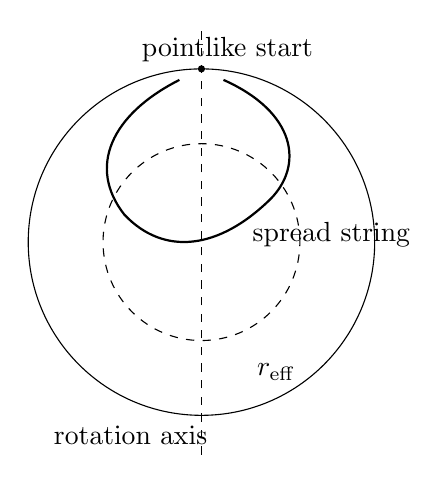
\begin{tikzpicture}[scale=1.0]
\draw (0,0) circle (2.2);
\draw[dashed] (0,-2.7) -- (0,2.7);
\draw[dashed] (0,0) circle (1.25);
\fill (0,2.2) circle (1.3pt);
\draw[thick]
(-0.28,2.06)
.. controls (-1.15,1.62) and (-1.45,0.95) .. (-0.98,0.35)
.. controls (-0.48,-0.18) and (0.22,-0.10) .. (0.88,0.55)
.. controls (1.30,0.98) and (1.20,1.65) .. (0.28,2.06);
\node at (0.33,2.45) {pointlike start};
\node at (1.65,0.10) {spread string};
\node at (0.95,-1.65) {$r_{\mathrm{eff}}$};
\node at (-0.90,-2.45) {rotation axis};
\end{tikzpicture}
\caption{Transcript-backed reconstruction of the string near the north pole, spreading out and behaving as if it were moving on a smaller effective sphere.}
\end{figure}

The moment of inertia is obtained by integrating the mass distribution against the square of the distance to the rotation axis. Once the string droops away from the north pole, some of its mass lies effectively closer to the axis than the original pointlike approximation assumed. The total mass has not changed, but the moment of inertia has become smaller:
\begin{equation}
I_{\mathrm{eff}}<mr^2.
\end{equation}
Equivalently, one may say that the motion behaves as if the string were a point particle on a smaller sphere,
\begin{equation}
E\sim \frac{L^2}{2I_{\mathrm{eff}}}
=
\frac{L^2}{2m r_{\mathrm{eff}}^2},
\qquad
r_{\mathrm{eff}}<r.
\end{equation}

Now comes the renormalization-group logic. If we add a few modes, the string behaves as though it were moving on a slightly smaller sphere. If we add still more modes, the effective description must be applied again to that smaller sphere. Repeating the process drives the effective radius inward again and again. There is no stabilization. The geometry keeps changing as the cutoff is raised.

\subsection{Question \& Answer}

\paragraph{Question.} Why do strings on spheres fail even though point particles do not?

\paragraph{Answer.} Because curvature couples the center-of-mass motion to the string's extension. For a point particle there is only the center of mass, and the sphere simply supplies a fixed moment of inertia. For a string, the object spreads out as more modes are included. On a curved background that spread changes the effective moment of inertia, so the geometry seen by the string is not the one we started with. In flat space the center-of-mass motion decouples from the spread; on the sphere it does not.

That is the lecture's blunt verdict: strings on spheres are not good theories. The problem is not merely that the string is large. The problem is that the effective geometry keeps running and never reaches a limit.

\section{Effective Geometry, Ricci Flow, and the Einstein Equations}

Once the sphere has taught us what can go wrong, the lecture immediately generalizes the lesson. A background geometry is described by its metric tensor \(g_{\mu\nu}(x)\), and as the cutoff is changed, the spread-out string sees an effective geometry that need not coincide with the original one.

\begin{figure}[h]
\centering

\includegraphics[width=0.72\textwidth]{lecture_09_figure_03.png}
\caption{Metric tensor notation on the board.}
\end{figure}

The board image shows only the beginning of the relevant equation, namely the appearance of \(g_{\mu\nu}(x)\) and the start of a change law. The lecture itself determines the content. The change in the effective geometry must vanish in flat space, so it must be built from curvature; and since the left-hand side is a symmetric rank-two tensor, the right-hand side must also be a symmetric rank-two tensor. The simplest such object is the Ricci tensor \(R_{\mu\nu}\). Thus the cutoff flow takes the schematic form
\begin{equation}
\delta g_{\mu\nu}(x)\propto -\,R_{\mu\nu}(x),
\end{equation}
or, in the logarithmic cutoff language used in the lecture,
\begin{equation}
\frac{d g_{\mu\nu}}{d\log \Lambda}\propto -\,R_{\mu\nu}.
\end{equation}
The minus sign is fixed heuristically by the sphere example: positive curvature pushes the effective sphere inward.

\begin{definition}
A stable string background, in the sense of this lecture, is a fixed point of the cutoff flow: as more and more modes are included, the effective geometry stops changing.
\end{definition}

Therefore the fixed-point condition is simply
\begin{equation}
R_{\mu\nu}=0.
\end{equation}
Such spaces are called Ricci flat. Flat space is the simplest example, but not the only one.

Susskind then springs the main payoff. Ricci flatness is not merely a geometric curiosity; it is the vacuum Einstein equation. The blackboard writes the Einstein tensor in the usual form:

\begin{figure}[h]
\centering

\includegraphics[width=0.80\textwidth]{lecture_09_figure_04.png}
\caption{Einstein tensor written in terms of curvature and stress tensor.}
\end{figure}

\begin{equation}
G_{\mu\nu}=R_{\mu\nu}-\frac{1}{2}g_{\mu\nu}R=T_{\mu\nu}.
\end{equation}
In vacuum we set \(T_{\mu\nu}=0\), so
\begin{equation}
G_{\mu\nu}=0.
\end{equation}
Taking the trace gives, in any relevant spacetime dimension \(D>2\),
\begin{equation}
g^{\mu\nu}G_{\mu\nu}
=
R-\frac{D}{2}R
=
0,
\end{equation}
hence \(R=0\). Substituting back, we obtain
\begin{equation}
R_{\mu\nu}=0.
\end{equation}

So the consistency condition for string propagation reproduces the vacuum Einstein equations. We did not put gravity in by hand at this stage; it emerged from the requirement that the continuum limit exist.

\begin{remark}
The lecture also notes that this spacetime condition is closely tied to conformal invariance on the worldsheet. For the present discussion the spacetime picture is enough: the cutoff flow must reach a fixed point.
\end{remark}

One caveat is inserted late, exactly in the lecture's rhythm. Ricci flatness is not the whole story. The independence of the cutoff really works only in the critical dimension: \(10\) for the superstring and \(26\) for the bosonic string.

\section{Compactification and Toroidal Backgrounds}

Only after the gravity payoff does the lecture turn to the practical question: what do we do with \(10\) or \(26\) dimensions? The answer is compactification. We do not remove the extra dimensions; we make them small enough that coarse-grained observers do not detect them as ordinary directions of motion.

The lecture takes the extra dimensions to be spatial. More than one time direction is set aside, not because one has proved an abstract impossibility in every imaginable framework, but because the simple and controllable theories under discussion do not make sense that way. Spatial compactification, by contrast, is concrete and calculable.

The elementary model is a line with a small circular direction attached to each point: macroscopically one sees only the line, while sufficiently small probes can move around the hidden circle. Periodic identification makes this precise.

\begin{figure}[h]
\centering
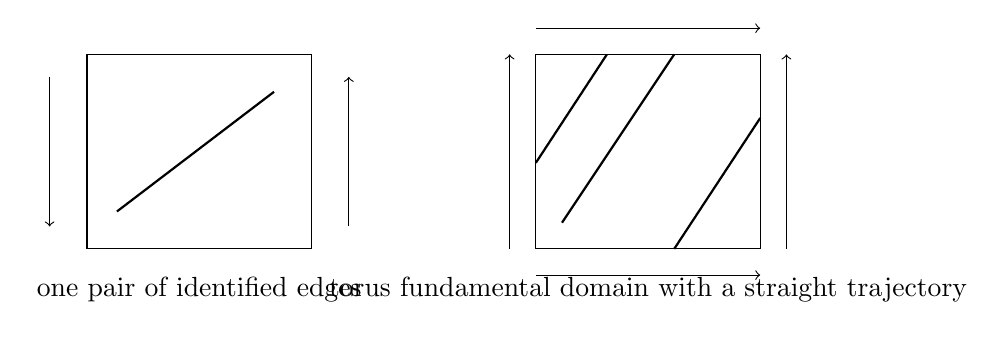
\begin{tikzpicture}[scale=0.95]
\draw (-6,-1.3) rectangle (-3,1.3);
\draw[->] (-6.5,1.0) -- (-6.5,-1.0);
\draw[->] (-2.5,-1.0) -- (-2.5,1.0);
\draw[thick] (-5.6,-0.8) -- (-3.5,0.8);
\node at (-4.5,-1.85) {one pair of identified edges};

\draw (0,-1.3) rectangle (3,1.3);
\draw[->] (0,1.65) -- (3,1.65);
\draw[->] (0,-1.65) -- (3,-1.65);
\draw[->] (-0.35,-1.3) -- (-0.35,1.3);
\draw[->] (3.35,-1.3) -- (3.35,1.3);
\draw[thick] (0.35,-0.95) -- (1.85,1.3);
\draw[thick] (1.85,-1.3) -- (3.0,0.45);
\draw[thick] (0.0,-0.15) -- (0.95,1.3);
\node at (1.5,-1.85) {torus fundamental domain with a straight trajectory};
\end{tikzpicture}
\caption{Transcript-backed reconstruction of periodic identification: first a cylinder, then a torus presented as a rectangle with opposite sides identified.}
\end{figure}

A torus here is a topology, not the bagel-shaped surface embedded in three-dimensional space. The rectangle with opposite sides identified is already the torus in the mathematical sense relevant to the lecture. Its virtue is precisely that it is easy to control. The identified fundamental domain can be given a flat metric, and therefore it is Ricci flat. This makes toroidal compactification the simplest safe compactification for string theory.

The lecture then goes one step further and asks how many inequivalent flat tori there are. At the level needed here, one should think of three parameters: the overall size, the aspect ratio, and a shear or twist before identification.

\begin{figure}[h]
\centering
\begin{tikzpicture}[scale=1.0]
\draw (0,0) rectangle (3,2);
\draw[<->] (0,-0.35) -- (3,-0.35);
\draw[<->] (-0.35,0) -- (-0.35,2);
\node at (1.5,-0.7) {width};
\node[rotate=90] at (-0.75,1.0) {height};

\draw (5,0) -- (8,0) -- (8.9,2) -- (5.9,2) -- cycle;
\draw[dashed] (5,0) -- (5.9,2);
\draw[<->] (5,2.35) -- (5.9,2.35);
\node at (6.8,2.7) {twist};
\end{tikzpicture}
\caption{A flat torus described by its fundamental domain: overall size, aspect ratio, and twist. The lecture uses the names K\"ahler modulus, complex-structure modulus, and Dehn twist in a loose explanatory sense.}
\end{figure}

The lecture briefly mentions more complicated Ricci-flat compactifications, especially Calabi--Yau manifolds, but the main pedagogical point is already visible on the torus. Tori are flat, hence Ricci flat, hence mathematically good backgrounds for strings. They are not realistic enough to describe the actual world, but they are solvable enough to expose the essential physics.

\section{Circle Compactification, Winding States, and T-Duality}

The final movement of the lecture specializes to the simplest compactification: one noncompact direction together with one compact circle of radius \(R\). This is the place where geometry becomes a spectral question.

The board first recalls the massless-particle relation:

\begin{figure}[h]
\centering

\includegraphics[width=0.72\textwidth]{lecture_09_figure_05.png}
\caption{Massless energy as the magnitude of momentum.}
\end{figure}

\begin{equation}
E=c|P|.
\end{equation}
Later, as is standard in this part of the discussion, the lecture effectively sets \(c=\hbar=1\).

Momentum along a periodic direction is quantized. If the circumference is \(2\pi R\), then the momentum around the circle behaves like angular momentum divided by \(R\), and so
\begin{equation}
p_c R = n\hbar.
\end{equation}
In units with \(\hbar=1\),
\begin{equation}
p_c=\frac{n}{R}, \qquad n\in \mathbb{Z}.
\end{equation}
From the lower-dimensional point of view, momentum in the compact direction looks like rest mass. Thus the Kaluza--Klein spectrum is
\begin{equation}
m_n=\frac{|n|}{R}.
\end{equation}

String theory adds a genuinely new possibility. A closed string can wrap around the compact circle. If we choose units in which the string tension is \(1\), the mass of a wound string is proportional to its length, and therefore to the radius of the circle:
\begin{equation}
m_w=|w|R,
\end{equation}
where \(w\in\mathbb{Z}\) is the winding number.

These two spectra are complementary:
\begin{align}
m_n &= \frac{|n|}{R},\\
m_w &= |w|R.
\end{align}
If \(R\) is small, the Kaluza--Klein levels are widely spaced and the winding levels are closely spaced. If \(R\) is large, the situation is reversed.

\begin{figure}[h]
\centering
\begin{tikzpicture}[scale=0.95]
\draw[->] (0,0) -- (0,4.6);
\foreach \y/\lab in {0/0,1.2/{1/R},2.4/{2/R},3.6/{3/R}}
{
\draw (-0.16,\y) -- (0.16,\y);
\node[left] at (-0.2,\y) {$\lab$};
}
\node at (0,-0.55) {Kaluza--Klein};

\draw[->] (5,0) -- (5,4.6);
\foreach \y/\lab in {0/0,1.2/{R},2.4/{2R},3.6/{3R}}
{
\draw (4.84,\y) -- (5.16,\y);
\node[right] at (5.2,\y) {$\lab$};
}
\node at (5,-0.55) {winding};
\end{tikzpicture}
\caption{Transcript-backed mass ladders for momentum modes and winding modes. Their exchange under \(R\leftrightarrow 1/R\) is the spectral seed of T-duality.}
\end{figure}

\subsection{Question \& Answer}

\paragraph{Question.} Can winding states be absent if we start without them?

\paragraph{Answer.} Not in a theory of closed strings. The lecture answers this dynamically rather than axiomatically. Start with a closed string of zero net winding. Stretch it around the compact direction so that one segment effectively winds one way and another segment winds the other way. The total winding is still zero. But the basic interaction in string theory is rearrangement: a single connected string can reconnect into two disconnected closed strings. After this rearrangement one obtains two separate particles with opposite winding numbers. Throw one far away and, locally, one is left with a winding state. So winding sectors are forced on us by the dynamics itself, just as charged particle--antiparticle pairs are forced on us in ordinary field theory.

Now the surprise. If we exchange
\begin{equation}
R \longleftrightarrow \frac{1}{R},
\qquad
n \longleftrightarrow w,
\end{equation}
the two spectra are interchanged and the set of masses is unchanged. At the special point \(R=1\) in these units, the two ladders coincide. More generally, shrinking the circle past this scale does not produce an essentially new closed-string theory; it produces the dual description of a larger circle. This is T-duality.

The lecture emphasizes that this is stronger than a cute coincidence of a few mass formulas. In a theory of closed strings, the full theory---spectrum, amplitudes, and interactions---is symmetric under the exchange of momentum and winding. That is a specifically stringy phenomenon. Point particles on a compact circle do not possess winding states and therefore do not possess this duality.

The final moral is geometric. The size of a compact direction can often be read, at least partly, from the spectrum of excitations. But string theory also teaches us that geometry is not always uniquely recoverable from the spectrum. Very small circles and very large circles can describe the same physics.

\section{Summary}

The lecture begins with a consistency question and ends with a duality. A point particle on a smooth curved space has a well-defined continuum limit. A string on a curved space need not. On the sphere, zero-point spreading lowers the effective moment of inertia and drives the background under a cutoff flow. The stable fixed points of that flow satisfy \(R_{\mu\nu}=0\), and this is precisely the vacuum Einstein equation. In this sense gravity is not added to string theory from outside; it is forced by consistency.

Only after that foundation is in place does compactification enter. Extra spatial dimensions can be hidden by periodic identification, and flat tori are the simplest Ricci-flat backgrounds on which strings can propagate sensibly. On a compact circle the spectrum splits into Kaluza--Klein momentum modes and stringy winding modes, with masses proportional to \(1/R\) and \(R\), respectively. Their exchange under \(R\leftrightarrow 1/R\) is T-duality, the final reminder that in string theory geometry is something we discover through spectra, not something we simply assume once and for all.